A tube of mass $M$ and length $\ell$ is free to swing around a pivot at one end. A mass $m$ is positioned inside the (frictionless) tube at this end. The tube is held horizontal and then released (see Fig. 1.5). Let $\eta$ be the fraction of the tube that the mass has traversed by the time the tube becomes vertical. Does $\eta$ depend on $\ell$?

\begin{center}
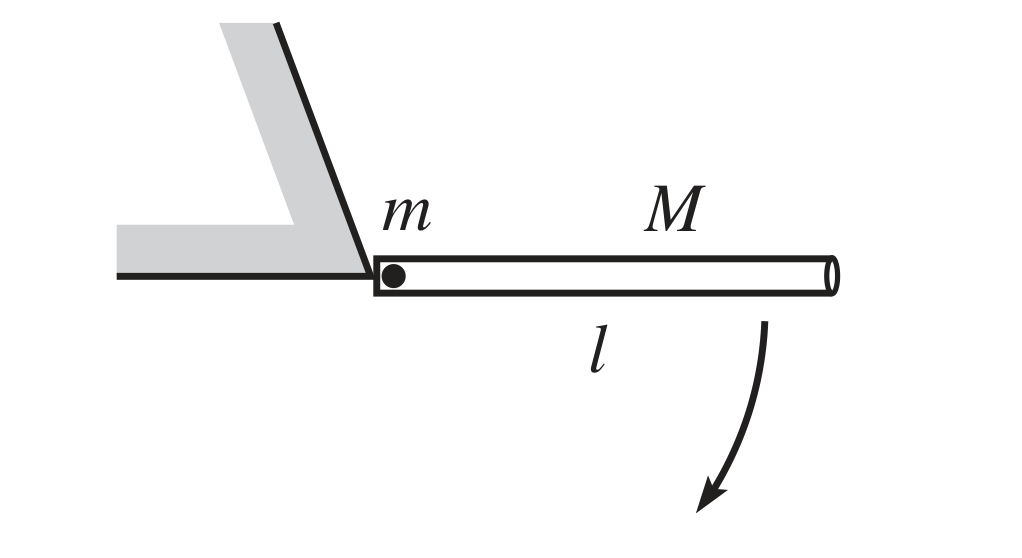
\includegraphics[width=\linewidth]{figures/qfig1.png}

Fig. 1.5
\end{center}